\documentclass[11pt]{charter}

% El títulos de la memoria, se usa en la carátula y se puede usar el cualquier lugar del documento con el comando \ttitle
\titulo{Solución Georeferenciada de monitoreo de ganado} 

% Nombre del posgrado, se usa en la carátula y se puede usar el cualquier lugar del documento con el comando \degreename
%\posgrado{Carrera de Especialización en Sistemas Embebidos} 
\posgrado{Carrera de Especialización en Internet de las Cosas} 
%\posgrado{Carrera de Especialización en Intelegencia Artificial}
%\posgrado{Maestría en Sistemas Embebidos} 
%\posgrado{Maestría en Internet de las cosas}

% Tu nombre, se puede usar el cualquier lugar del documento con el comando \authorname
\autor{Christian Canaan Castro Botek} 

% El nombre del director y co-director, se puede usar el cualquier lugar del documento con el comando \supname y \cosupname y \pertesupname y \pertecosupname
\director{Nombre del Director}
\pertenenciaDirector{pertenencia} 
% FIXME:NO IMPLEMENTADO EL CODIRECTOR ni su pertenencia
\codirector{} % si queda vacio no se deberíá incluir 
\pertenenciaCoDirector{}

% Nombre del cliente, quien va a aprobar los resultados del proyecto, se puede usar con el comando \clientename y \empclientename
\cliente{Mg. Ing. Osvaldo P. Ivani}
\empresaCliente{Smartium}

% Nombre y pertenencia de los jurados, se pueden usar el cualquier lugar del documento con el comando \jurunoname, \jurdosname y \jurtresname y \perteunoname, \pertedosname y \pertetresname.
\juradoUno{Nombre y Apellido (1)}
\pertenenciaJurUno{pertenencia (1)} 
\juradoDos{Nombre y Apellido (2)}
\pertenenciaJurDos{pertenencia (2)}
\juradoTres{Nombre y Apellido (3)}
\pertenenciaJurTres{pertenencia (3)}
 
\fechaINICIO{25 de Agosto de 2020}		%Fecha de inicio de la cursada de GdP \fechaInicioName
\fechaFINALPlanificacion{29 de Septiembre de 2020} 	%Fecha de final de cursada de GdP
\fechaFINALTrabajo{20 de Julio de 2021}		%Fecha de defensa pública del trabajo final


\begin{document}

\maketitle
\thispagestyle{empty}
\pagebreak


\thispagestyle{empty}
{\setlength{\parskip}{0pt}
\tableofcontents{}
}
\pagebreak


\section{Registros de cambios}
\label{sec:registro}


\begin{table}[ht]
\label{tab:registro}
\centering
\begin{tabularx}{\linewidth}{@{}|c|X|c|@{}}
\hline
\rowcolor[HTML]{C0C0C0} 
Revisión & \multicolumn{1}{c|}{\cellcolor[HTML]{C0C0C0}Detalles de los cambios realizados} & Fecha      \\ \hline
1.0      & Creación del documento                                          & 25/08/2020 \\ \hline
1.1      & Se completaron los puntos del 1 al 6                                                                 & 06/09/2020 \\ \hline
1.2      & Otro ejemplo \newline
		   Con texto partido \newline
		   En varias líneas \newline
		   A propósito                                                     & dd/mm/aaaa \\ \hline
\end{tabularx}
\end{table}

\pagebreak



\section{Acta de constitución del proyecto}
\label{sec:acta}

\begin{flushright}
Buenos Aires, \fechaInicioName
\end{flushright}

\vspace{2cm}

Por medio de la presente se acuerda con el Ing. \authorname\hspace{1px} que su Trabajo Final de la \degreename\hspace{1px} se titulará ``\ttitle'', consistirá esencialmente en el prototipo preliminar de un sistema georreferenciado de monitoreo de ganado, y tendrá un presupuesto preliminar estimado de 600 hs de trabajo y \textcolor{red}{\$XXX}, con fecha de inicio \fechaInicioName\hspace{1px} y fecha de presentación pública \fechaFinalName.

Se adjunta a esta acta la planificación inicial.

\vfill

% Esta parte se construye sola con la información que hayan cargado en el preámbulo del documento y no debe modificarla
\begin{table}[ht]
\centering
\begin{tabular}{ccc}
\begin{tabular}[c]{@{}c@{}}Ariel Lutenberg \\ Director posgrado FIUBA\end{tabular} & \hspace{2cm} & \begin{tabular}[c]{@{}c@{}}\clientename \\ \empclientename \end{tabular} \vspace{2.5cm} \\ 
\multicolumn{3}{c}{\begin{tabular}[c]{@{}c@{}} \supname \\ Director del Trabajo Final\end{tabular}} \vspace{2.5cm} \\
%\begin{tabular}[c]{@{}c@{}}\jurunoname \\ Jurado del Trabajo Final\end{tabular}     &  & \begin{tabular}[c]{@{}c@{}}\jurdosname\\ Jurado del Trabajo Final\end{tabular}  \vspace{2.5cm}  \\
%\multicolumn{3}{c}{\begin{tabular}[c]{@{}c@{}} \jurtresname\\ Jurado del Trabajo Final\end{tabular}} \vspace{.5cm}                                                                     
\end{tabular}
\end{table}




\section{Descripción técnica-conceptual del proyecto a realizar}
\label{sec:descripcion}


La ganaderia argentina esta pasando por un cambio estructural con el objetivo de ajustarse a la demanda interna y recuperar al mismo tiempo el protagonismo internacional. Producto de esto, Los últimos años creció 10\% la producción de las cuatro carnes hasta alcanzar los 6 millones de toneladas representando la carne vacuna el 50\% de la oferta. Actualmente la Argentina paso a ocupar el 5to puesto en exportaciones de carne bovina, los cuales el 75\% de los envios fueron a China, generando asi un total de u\$s 1.000 millones. Bajo este panorama, los avances tecnologicos innovadores se afianzan con el objetivo de lograr producciones mas eficientes, controladas y previsorias que contribuyan y disparen los beneficios del mercado. 

Bajo este escenario se espera implementar un sistema autonomo, de bajo costo y consumo que permita recopilar, almacenar, procesar y visualizar la posición de determinadas cabezas de ganado a través de GPS y que opere bajo una red LoRaWAN. Adicionalmente a esto, toda la informacion recolectada debera ser almacenada y posteriormente procesada para ser visualizada en una aplicacion permitiendo al agricultor/criador tener a disposicion un historial de ubicaciones de sus animales en tiempo real. El sistema debe ser escalable y operar con baterias, enviando periodicamente la posicion de la cabeza de ganado. En la figura 1. se puede observar la composicion basica del sistema. 



\vspace{25px}

\begin{figure}[htpb]
\centering 
\includegraphics[width=.9\textwidth]{./Figuras/Diagrama2.png}
\caption{Diagrama en bloques del sistema}
\label{fig:diagBloques}
\end{figure}

\vspace{25px}

El objetivo principal es la implementacion de un pequeño dispositivo que pueda ser colocado en un collar lo suficientemente comodo para el animal y que sea capaz de tomar la posición GPS bajo un sistema que comprenda un microcontrolador y hardware de bajo consumo almientado con baterias recargables. Al mismo tiempo deberá ser capaz de transmitir la posición y telemetria interna del dispositivo tales como ID, nivel de bateria, he intensidad de la señal haciendo uso de una red LoRaWAN que permitirá guardar los datos en la nube para su posterior procesamiento. 

%El equipo deberá alimentarse con baterias recargables incorporando un cargador "onboard" que permita la recarga por micro-USB y ser resistente a condiciones ambientales extremas. 

El proyecto permitirá al agricultor/criador, tener un total control de su ganado, permitiendole visualizar en tiempo real la ubicacion de los mismos, disponer de un historial de movimiento y ubicacion de cada animal, vista total de los limites de su terreno, deducir estado de pastizales en su territorio en base a un historial de movimiento de su ganado, deducir estado de salud de sus animales y control de robo o atentado; todos fuertes contrubiyentes a aumentar la calidad, eficiencia y total control de su ganado. 


\section{Identificación y análisis de los interesados}
\label{sec:interesados}


\begin{table}[ht]
%\caption{Identificación de los interesados}
%\label{tab:interesados}
\begin{tabularx}{\linewidth}{@{}|l|X|X|l|@{}}
\hline
\rowcolor[HTML]{C0C0C0} 
Rol           & Nombre y Apellido & Organización 	& Puesto 	\\ \hline
%Auspiciante   &                   &              	&        	\\ \hline
Cliente       & \clientename      &\empclientename	& Gerente de Ingenieria       	\\ \hline
%Impulsor      &                   &              	&        	\\ \hline
Responsable   & \authorname       & FIUBA        	& Alumno 	\\ \hline
Colaboradores & Ing. Jhonattan Camargo                & Smartium             	& Project Manager       	\\ \hline
Orientador    & \supname	      & \pertesupname 	& Director	Trabajo final \\ \hline
%Equipo        & miembro1 \newline 
%				miembro2          &              	&        	\\ \hline
%Opositores    &                   &              	&        	\\ \hline
Usuario final & -                  & Criador que desee implementar una solución tecnológica en su ganado             	&  -      	\\ \hline
\end{tabularx}
\end{table}

El Mg. Ing. Osvaldo P. Ivani tiene muchos conocimientos técnicos y es un gran guia para la elaboración del proyecto pero no dispone de mucho tiempo por tener una gran responsabilidad laboral. 

El Esp. Ing. Jhonattan Camargo posee conocimientos del tema y será de gran ayuda para solventar dudas técnicas y del proyecto, tambien tiene una agenda ocupada y no dispone de mucho tiempo.



\section{1. Propósito del proyecto}
\label{sec:proposito}

El proposito de este proyecto es desarrollar el prototipo de un sistema autonomo capaz de transmitir la ubicación exacta de una cabeza de ganado y a partir de allí implementar una aplicación capaz de usar estos datos para relevar en tiempo real y de forma remota mas información al criador sobre el estado de su su campo y su ganado. 

\section{2. Alcance del proyecto}
\label{sec:alcance}

EL alcance de este proyecto incluirá un prototipo de hardware capaz de transmitir la posicion a traves de la red de comunicacion LoRa y el desarrollo de una aplicacion integrada con AWS cloud capaz de utilizar estos datos para mostrarlos en pantalla. Al mismo tiempo no implicara la conexion desde el Gateway hasta el servidor de Aplicacion ni la capacitacion del usuario para hacer uso de la aplicacion. 


\section{3. Supuestos del proyecto}
\label{sec:supuestos}

Para el cumplimiento de este proyecto se supone que: 

\begin{itemize}
\item Se dispondra del tiempo y espacio para realizar distintas pruebas.
\item Habran recursos economicos para la construcción del hardware.
\item Los tiempos fabricacion estaran dentro de los margenes habituales.
\item Existirá comunicacion permanente con el cliente para solventar dudas.
\item Los tiempos de autonomia del hardware estaran basandos en cálculos pesimistas y no en ensayos controlados.
\end{itemize}


\section{4. Requerimientos}
\label{sec:requerimientos}

Los requerimientos del proyecto fueron convenidos por ambas partes a traves del documento inicial de presentación del proyecto y distintas reuniones coordinadas. 


\begin{enumerate}
\item Requerimientos generales del proyecto:
	\begin{enumerate}
	\item Deadline 20 julio 2021
	\item Entregable prototipo de hardware funcional y prototipo de aplicacion con funcion de visualizacion de terreno y ubicación en tiempo real. 
	\end{enumerate}
\item Requerimientos funcionales del sistema:
	\begin{enumerate}
	\item Hardware:
		\begin{enumerate}
		\item Hardware tipo collar con un peso no superior a los 250gr y protección IP46 o superior.
		\item Envio de coordenadas GPS a traves de enlace de radiofrecuencia LoRaWAN en banda AU915.
		\item Bajo consumo con autonomia minima de 1 año.
		\item Entrada de recarga de bateria por micro-USB.
		\item Bajo costo.
		\end{enumerate}
	\item Software:
		\begin{enumerate}
		\item Almacenamiento de la información recolectada.
		\item Validación de usuario con la plataforma Smartium.
		\item Escalabilidad a nivel de sooftware para nuevos collares.
		\item Creación y asociación de nuevos animales donde se podran cargar identificador unico, tipo, nombre, fecha, etc.
		\item Calculos de distancia recorrida por el animal de forma diaria, cada tres dias y semanales.
		\item Creacion de zonas georeferenciadas para establecer si un animal está fuera del territorio.
		\item Viasualización de la última posición de los animales asociados a un usuario junto con su respectivo historial de ubicación.
		\item Plataforma compatible con AWS Cloud.
		\item Bajo tráfico de datos.
		\end{enumerate}
	\end{enumerate}
\item Requerimientos de documentación:
	\begin{enumerate}
	\item Elaboración de un informe de avance del proyecto.
	\item Elaboración de informe de puesta en marcha.
	\end{enumerate}	
\end{enumerate}



%\section{Historias de usuarios (\textit{Product backlog})}
%\label{sec:backlog}

%\begin{consigna}{red}
%Descripción: En esta sección se deben incluir las historias de usuarios y su ponderación (\textit{history points}). Recordar que las historias de usuarios son descripciones cortas y simples de una característica contada desde la perspectiva de la persona que desea la nueva capacidad, generalmente un usuario o cliente del sistema. La ponderación es un número entero que representa el tamaño de la historia comparada con otras historias de similar tipo.
%\end{consigna}

\section{5. Entregables principales del proyecto}
\label{sec:entregables}


\begin{itemize}
\item Planificación del trabajo final.
\item Prototipo funcional del hardware y software de aplicación.
\item Código fuente.
\item Diagrama esquematico.
\item Informe final.

\end{itemize}

\section{6. Desglose del trabajo en tareas}
\label{sec:wbs}


\begin{enumerate}
\item Análisis inicial (130)
	\begin{enumerate}
	\item Lectura de referencias bibliograficas (60)
	\item Introducción a herramientas necesarias (30)
	\item Elaboración de la planificación del proyecto (40)
	\end{enumerate}
\item Diseño de Hardware (165)
	\begin{enumerate}
	\item Diseño estructura del sistema (40)
	\item Diseño de esquematico preliminar (15)
	\item Selección de componentes (15)
	\item Elaboración de esquemático (15)
	\item Análisis de consumo (10)
	\item Diseño de PCB (20)
	\item Diseño del prototipo físico (20)
	\item Elaboración de protocolos de transmisión y confirmación de envío de datos a la red LoRaWAN (30)
	\end{enumerate}
\item Producción (80)
	\begin{enumerate}
	\item Fabricación del PCB (20)
	\item Montaje del circuito (20)
	\item Fabricación del prototipo (40)
	\end{enumerate}
\item Testing (70)
	\begin{enumerate}
	\item Comprobación de funcionamiento del circuito (20)
	\item Ensayo y medición de consumo (20)
	\item Ensayo de comunicación con la red LoRaWAN (20)
	\item Checkeo de la correcta llegada de datos al Cloud (10)
	\end{enumerate}
\item Aplicación (155)
	\begin{enumerate}
	\item Selección de estrategia y entorno de programación (20)
	\item Comunicación y permisos con la nube (20)
	\item Desarrollo del login de usuario (10)
	\item Comprobación de comunicación y login correctos (5)
        \item Desarrollo de interfaz de usuario (60)
	\item Desarrollo de algoritmos de historial de ubicación (40)
	\end{enumerate}
\item Ensayos sobre aplicación (20)
	\begin{enumerate}
	\item Pruebas sobre la aplicación (10)
	\item Corrección de errores y ajustes menores (10)
	\end{enumerate}
\item Finalización (50)
	\begin{enumerate}
	\item Elaboración de documentación (20)
	\item Elaboración de la presentación del proyecto final (20)
	\item Cierre del proyecto (10)
	\end{enumerate}
\end{enumerate}

Cantidad total de horas: (670)
 


\section{7. Diagrama de Activity On Node}
\label{sec:AoN}

\begin{consigna}{red}
Armar el AoN a partir del WBS definido en la etapa anterior. 

%La figura \ref{fig:AoN} fue elaborada con el paquete latex tikz y pueden consultar la siguiente referencia \textit{online}:

%\url{https://www.overleaf.com/learn/latex/LaTeX_Graphics_using_TikZ:_A_Tutorial_for_Beginners_(Part_3)\%E2\%80\%94Creating_Flowcharts}

\end{consigna}

\begin{figure}[htpb]
\centering 
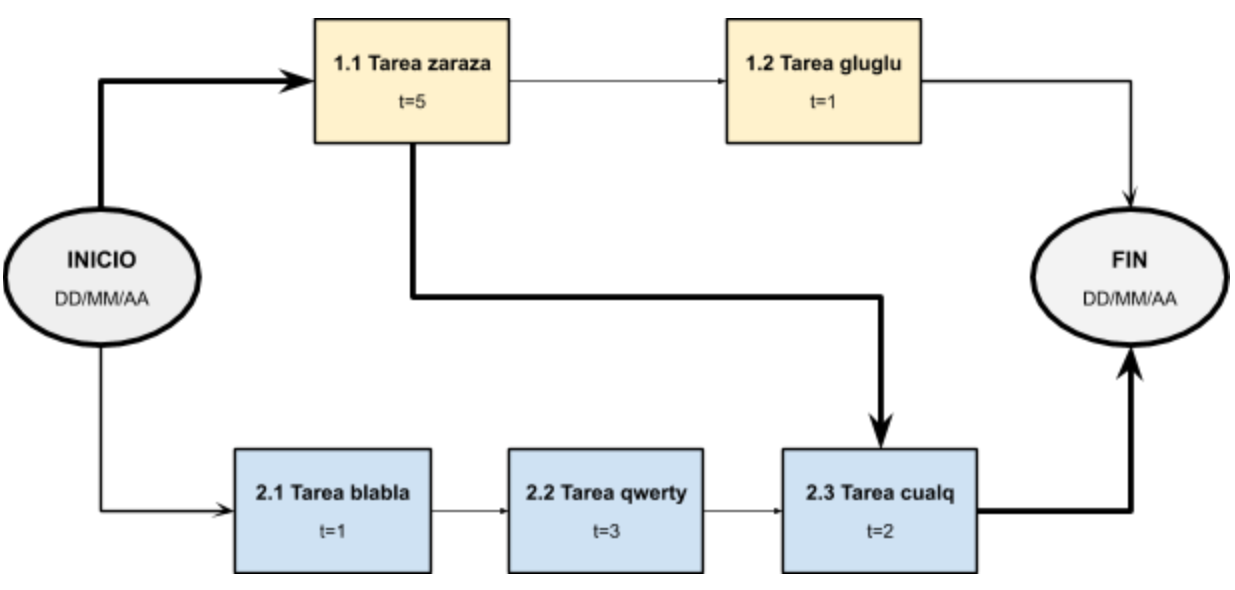
\includegraphics[width=.8\textwidth]{./Figuras/AoN.png}
\caption{Diagrama en \textit{Activity on Node}}
\label{fig:AoN}
\end{figure}

Indicar claramente en qué unidades están expresados los tiempos.
De ser necesario indicar los caminos semicríticos y analizar sus tiempos mediante un cuadro.
Es recomendable usar colores y un cuadro indicativo describiendo qué representa cada color, como se muestra en el siguiente ejemplo:



\section{8. Diagrama de Gantt}
\label{sec:gantt}

\begin{consigna}{red}
Utilizar el software Gantter for Google Drive o alguno similar para dibujar el diagrama de Gantt.

Existen muchos programas y recursos \textit{online} para hacer diagramas de gantt, entre las cuales destacamos:

\begin{itemize}
\item Planner
\item GanttProject
\item Trello + \textit{plugins}. En el siguiente link hay un tutorial oficial: \\ \url{https://blog.trello.com/es/diagrama-de-gantt-de-un-proyecto}
\item Creately, herramienta online colaborativa. \\\url{https://creately.com/diagram/example/ieb3p3ml/LaTeX}
\item Se puede hacer en latex con el paquete \textit{pgfgantt}\\ \url{http://ctan.dcc.uchile.cl/graphics/pgf/contrib/pgfgantt/pgfgantt.pdf}
\end{itemize}

Pegar acá una captura de pantalla del diagrama de Gantt, cuidando que la letra sea suficientemente grande como para ser legible. 
Si el diagrama queda demasiado ancho, se puede pegar primero la ``tabla'' del Gantt y luego pegar la parte del diagrama de barras del diagrama de Gantt.

Configurar el software para que en la parte de la tabla muestre los códigos del EDT (WBS).\\
Configurar el software para que al lado de cada barra muestre el nombre de cada tarea.\\
Revisar que la fecha de finalización coincida con lo indicado en el Acta Constitutiva.

En la figura \ref{fig:gantt}, se muestra un ejemplo de diagrama de gantt realizado con el paquete de \textit{pgfgantt}. En la plantilla pueden ver el código que lo genera y usarlo de base para construir el propio.

\begin{figure}[htbp]
\begin{center}
\begin{ganttchart}{1}{12}
  \gantttitle{2020}{12} \\
  \gantttitlelist{1,...,12}{1} \\
  \ganttgroup{Group 1}{1}{7} \\
  \ganttbar{Task 1}{1}{2} \\
  \ganttlinkedbar{Task 2}{3}{7} \ganttnewline
  \ganttmilestone{Milestone o hito}{7} \ganttnewline
  \ganttbar{Final Task}{8}{12}
  \ganttlink{elem2}{elem3}
  \ganttlink{elem3}{elem4}
\end{ganttchart}
\end{center}
\caption{Diagrama de gantt de ejemplo}
\label{fig:gantt}
\end{figure}

\end{consigna}

\section{9. Matriz de uso de recursos de materiales}
\label{sec:recursos}


\begin{table}
\label{tab:recursos}
\centering
\begin{tabularx}{\linewidth}{@{}|c|X|X|X|X|c|@{}}
\hline
\cellcolor[HTML]{C0C0C0} & \cellcolor[HTML]{C0C0C0} & \multicolumn{4}{c|}{\cellcolor[HTML]{C0C0C0}Recursos requeridos (horas)} \\ \cline{3-6} 
\multirow{-2}{*}{\cellcolor[HTML]{C0C0C0}\begin{tabular}[c]{@{}c@{}}Código\\ WBS\end{tabular}} & \multirow{-2}{*}{\cellcolor[HTML]{C0C0C0}\begin{tabular}[c]{@{}c@{}}Nombre \\ tarea\end{tabular}} & Material 1 & Material 2 & Material 3 & Material 4 \\ \hline
 &  &  &  &  &  \\ \hline
 &  &  &  &  &  \\ \hline
 &  &  &  &  &  \\ \hline
 &  &  &  &  &  \\ \hline
 &  &  &  &  &  \\ \hline
 &  &  &  &  &  \\ \hline
 &  &  &  &  &  \\ \hline
 &  &  &  &  &  \\ \hline 
 &  &  &  &  &  \\ \hline
 &  &  &  &  &  \\ \hline
 &  &  &  &  &  \\ \hline
 &  &  &  &  &  \\ \hline
 &  &  &  &  &  \\ \hline
 &  &  &  &  &  \\ \hline
 &  &  &  &  &  \\ \hline
 &  &  &  &  &  \\ \hline
 &  &  &  &  &  \\ \hline
 &  &  &  &  &  \\ \hline
 &  &  &  &  &  \\ \hline
 &  &  &  &  &  \\ \hline
 &  &  &  &  &  \\ \hline
 &  &  &  &  &  \\ \hline
 &  &  &  &  &  \\ \hline
 &  &  &  &  &  \\ \hline 
 &  &  &  &  &  \\ \hline
 &  &  &  &  &  \\ \hline
 &  &  &  &  &  \\ \hline
 &  &  &  &  &  \\ \hline

\end{tabularx}%
\end{table}


\section{10. Presupuesto detallado del proyecto}
\label{sec:presupuesto}

\begin{consigna}{red}
Si el proyecto es complejo entonces separarlo en partes:
\begin{itemize}
\item Un total global, indicando el subtotal acumulado por cada una de las áreas.
\item El desglose detallado del subtotal de cada una de las áreas.
\end{itemize}

IMPORTANTE: No olvidarse de considerar los COSTOS INDIRECTOS.

\end{consigna}

\begin{table}[htpb]
\centering
\begin{tabularx}{\linewidth}{@{}|X|c|r|r|@{}}
\hline
\rowcolor[HTML]{C0C0C0} 
\multicolumn{4}{|c|}{\cellcolor[HTML]{C0C0C0}COSTOS DIRECTOS} \\ \hline
\rowcolor[HTML]{C0C0C0} 
Descripción &
  \multicolumn{1}{c|}{\cellcolor[HTML]{C0C0C0}Cantidad} &
  \multicolumn{1}{c|}{\cellcolor[HTML]{C0C0C0}Valor unitario} &
  \multicolumn{1}{c|}{\cellcolor[HTML]{C0C0C0}Valor total} \\ \hline
 &
  \multicolumn{1}{c|}{} &
  \multicolumn{1}{c|}{} &
  \multicolumn{1}{c|}{} \\ \hline
 &
  \multicolumn{1}{c|}{} &
  \multicolumn{1}{c|}{} &
  \multicolumn{1}{c|}{} \\ \hline
\multicolumn{1}{|l|}{} &
   &
   &
   \\ \hline
\multicolumn{1}{|l|}{} &
   &
   &
   \\ \hline
\multicolumn{3}{|c|}{SUBTOTAL} &
  \multicolumn{1}{c|}{} \\ \hline
\rowcolor[HTML]{C0C0C0} 
\multicolumn{4}{|c|}{\cellcolor[HTML]{C0C0C0}COSTOS INDIRECTOS} \\ \hline
\rowcolor[HTML]{C0C0C0} 
Descripción &
  \multicolumn{1}{c|}{\cellcolor[HTML]{C0C0C0}Cantidad} &
  \multicolumn{1}{c|}{\cellcolor[HTML]{C0C0C0}Valor unitario} &
  \multicolumn{1}{c|}{\cellcolor[HTML]{C0C0C0}Valor total} \\ \hline
\multicolumn{1}{|l|}{} &
   &
   &
   \\ \hline
\multicolumn{1}{|l|}{} &
   &
   &
   \\ \hline
\multicolumn{1}{|l|}{} &
   &
   &
   \\ \hline
\multicolumn{3}{|c|}{SUBTOTAL} &
  \multicolumn{1}{c|}{} \\ \hline
\rowcolor[HTML]{C0C0C0}
\multicolumn{3}{|c|}{TOTAL} &
   \\ \hline
\end{tabularx}%
\end{table}


\section{11. Matriz de asignación de responsabilidades}
\label{sec:responsabilidades}
\begin{consigna}{red}
Establecer la matriz de asignación de responsabilidades y el manejo de la autoridad completando la siguiente tabla:

\begin{table}[htpb]
\centering
\resizebox{\textwidth}{!}{%
\begin{tabular}{|c|c|c|c|c|c|}
\hline
\rowcolor[HTML]{C0C0C0} 
\cellcolor[HTML]{C0C0C0} &
  \cellcolor[HTML]{C0C0C0} &
  \multicolumn{4}{c|}{\cellcolor[HTML]{C0C0C0}Listar todos los nombres y roles del proyecto} \\ \cline{3-6} 
\rowcolor[HTML]{C0C0C0} 
\cellcolor[HTML]{C0C0C0} &
  \cellcolor[HTML]{C0C0C0} &
  Responsable &
  Orientador &
  Equipo &
  Cliente \\ \cline{3-6} 
\rowcolor[HTML]{C0C0C0} 
\multirow{-3}{*}{\cellcolor[HTML]{C0C0C0}\begin{tabular}[c]{@{}c@{}}Código\\ WBS\end{tabular}} &
  \multirow{-3}{*}{\cellcolor[HTML]{C0C0C0}Nombre de la tarea} &
  \authorname &
  \supname &
  Nombre de alguien &
  \clientename \\ \hline
 &  &  &  &  &  \\ \hline
 &  &  &  &  &  \\ \hline
 &  &  &  &  &  \\ \hline
\end{tabular}%
}
\end{table}

{\footnotesize
Referencias:
\begin{itemize}
	\item P = Responsabilidad Primaria
	\item S = Responsabilidad Secundaria
	\item A = Aprobación
	\item I = Informado
	\item C = Consultado
\end{itemize}
} %footnotesize

Una de las columnas debe ser para el Director, ya que se supone que participará en el proyecto.
A su vez se debe cuidar que no queden muchas tareas seguidas sin ``A'' o ``I''.

Importante: es redundante poner ``I/A'' o ``I/C'', porque para aprobarlo o responder consultas primero la persona debe ser informada.

\end{consigna}

\section{12. Gestión de riesgos}
\label{sec:riesgos}

\begin{consigna}{red}
a) Identificación de los riesgos (al menos cinco) y estimación de sus consecuencias:
 
Riesgo 1: detallar el riesgo (riesgo es algo que si ocurre altera los planes previstos)
\begin{itemize}
\item Severidad (S): mientras más severo, más alto es el número (usar números del 1 al 10).\\
Justificar el motivo por el cual se asigna determinado número de severidad (S).
\item Probabilidad de ocurrencia (O): mientras más probable, más alto es el número (usar del 1 al 10).\\
Justificar el motivo por el cual se asigna determinado número de (O). 
\end{itemize}   

Riesgo 2:
\begin{itemize}
\item Severidad (S): 
\item Ocurrencia (O):
\end{itemize}

Riesgo 3:
\begin{itemize}
\item Severidad (S): 
\item Ocurrencia (O):
\end{itemize}


b) Tabla de gestión de riesgos:      (El RPN se calcula como RPN=SxO)

\begin{table}[htpb]
\centering
\begin{tabularx}{\linewidth}{@{}|X|c|c|c|c|c|c|@{}}
\hline
\rowcolor[HTML]{C0C0C0} 
Riesgo & S & O & RPN & S* & O* & RPN* \\ \hline
       &   &   &     &    &    &      \\ \hline
       &   &   &     &    &    &      \\ \hline
       &   &   &     &    &    &      \\ \hline
       &   &   &     &    &    &      \\ \hline
       &   &   &     &    &    &      \\ \hline
\end{tabularx}%
\end{table}

Criterio adoptado: 
Se tomarán medidas de mitigación en los riesgos cuyos números de RPN sean mayores a...

Nota: los valores marcados con (*) en la tabla corresponden luego de haber aplicado la mitigación.

c) Plan de mitigación de los riesgos que originalmente excedían el RPN máximo establecido:
 
Riesgo 1: plan de mitigación (si por el RPN fuera necesario elaborar un plan de mitigación).
  Nueva asignación de S y O, con su respectiva justificación:
  - Severidad (S): mientras más severo, más alto es el número (usar números del 1 al 10).
          Justificar el motivo por el cual se asigna determinado número de severidad (S).
  - Probabilidad de ocurrencia (O): mientras más probable, más alto es el número (usar del 1 al 10).
          Justificar el motivo por el cual se asigna determinado número de (O).

Riesgo 2: plan de mitigación (si por el RPN fuera necesario elaborar un plan de mitigación).
 
Riesgo 3: plan de mitigación (si por el RPN fuera necesario elaborar un plan de mitigación).

\end{consigna}


\section{13. Gestión de la calidad}
\label{sec:calidad}

\begin{consigna}{red}
Para cada uno de los requerimientos del proyecto indique:
\begin{itemize} 
\item Req \#1: copiar acá el requerimiento.

Verificación y validación:

\begin{itemize}
\item Verificación para confirmar si se cumplió con lo requerido antes de mostrar el sistema al cliente. Detallar 
\item Validación con el cliente para confirmar que está de acuerdo en que se cumplió con lo requerido. Detallar  
\end{itemize}

\end{itemize}

Tener en cuenta que en este contexto se pueden mencionar simulaciones, cálculos, revisión de hojas de datos, consulta con expertos, mediciones, etc.

\end{consigna}

\section{14. Comunicación del proyecto}
\label{sec:comunicaciones}

El plan de comunicación del proyecto es el siguiente:

\begin{table}[htpb]
\centering
\begin{tabularx}{\linewidth}{@{}|X|C{2.4cm}|C{3cm}|C{1.8cm}|C{2cm}|C{2.1cm}|@{}}
\hline
\rowcolor[HTML]{C0C0C0} 
\multicolumn{6}{|c|}{\cellcolor[HTML]{C0C0C0}PLAN DE COMUNICACIÓN DEL PROYECTO}           \\ \hline
\rowcolor[HTML]{C0C0C0} 
¿Qué comunicar? & Audiencia & Propósito & Frecuencia & Método de comunicac. & Responsable \\ \hline
                &           &           &            &                      &             \\ \hline
                &           &           &            &                      &             \\ \hline
                &           &           &            &                      &             \\ \hline
                &           &           &            &                      &             \\ \hline
                &           &           &            &                      &             \\ \hline
\end{tabularx}
\end{table}

\section{15. Gestión de compras}
\label{sec:compras}

\begin{consigna}{red}
En caso de tener que comprar elementos o contratar servicios:
a) Explique con qué criterios elegiría a un proveedor.
b) Redacte el Statement of Work correspondiente.
\end{consigna}

\section{16. Seguimiento y control}
\label{sec:seguimiento}

\begin{consigna}{red}
Para cada tarea del proyecto establecer la frecuencia y los indicadores con los se seguirá su avance y quién será el responsable de hacer dicho seguimiento y a quién debe comunicarse la situación (en concordancia con el Plan de Comunicación del proyecto).

El indicador de avance tiene que ser algo medible, mejor incluso si se puede medir en \% de avance. Por ejemplo,se pueden indicar en esta columna cosas como ``cantidad de conexiones ruteadeas'' o ``cantidad de funciones implementadas'', pero no algo genérico y ambiguo como ``\%'', porque el lector no sabe porcentaje de qué cosa.

\end{consigna}

\begin{longtable}{|m{1cm}|m{3.5cm}|m{2.2cm}|m{2cm}|m{3cm}|m{1.5cm}|}
\hline
\rowcolor[HTML]{C0C0C0} 
\multicolumn{6}{|c|}{\cellcolor[HTML]{C0C0C0}SEGUIMIENTO DE AVANCE}                                                                       \\ \hline
\rowcolor[HTML]{C0C0C0} 
Tarea del WBS 			& Indicador de avance & Frecuencia de reporte & Resp. de seguimiento & Persona a ser informada & Método de comunic. \\ \hline
\endfirsthead

\hline
\rowcolor[HTML]{C0C0C0} 
\multicolumn{6}{c}{\cellcolor[HTML]{C0C0C0}SEGUIMIENTO DE AVANCE}                                                                       \\ \hline
\rowcolor[HTML]{C0C0C0} 
Tarea del WBS 			& Indicador de avance & Frecuencia de reporte & Resp. de seguimiento & Persona a ser informada & Método de comunic. \\ \hline
\endhead

\multicolumn{6}{c}{Continúa}
\endfoot

\endlastfoot

1.1	& Fecha de inicio  & Única vez al comienzo & \authorname & \clientename, \supname & email \\ \hline
2.1	& Avance de las subtareas  & Mensual mientras dure la tarea & \authorname & \clientename, \supname & email \\ \hline

\end{longtable}

\begin{table}[!htpb]
\centering
%\begin{tabularx}{\linewidth}{@{}|X|X|X|X|X|X|@{}}
\begin{tabularx}{\linewidth}{@{}|X|C{2.5cm}|C{3cm}|C{2cm}|C{2cm}|C{2.5cm}|@{}}
\hline
\rowcolor[HTML]{C0C0C0} 
\multicolumn{6}{|c|}{\cellcolor[HTML]{C0C0C0}SEGUIMIENTO DE AVANCE}                                                                       \\ \hline
\rowcolor[HTML]{C0C0C0} 
Tarea del WBS & Indicador de avance & Frecuencia de reporte & Resp. de seguimiento & Persona a ser informada & Método de comunic. \\ \hline
 &  &  &  &  &  \\ \hline
 &  &  &  &  &  \\ \hline
 &  &  &  &  &  \\ \hline
 &  &  &  &  &  \\ \hline
 &  &  &  &  &  \\ \hline
\end{tabularx}%
%}
\end{table}

\section{17. Procesos de cierre}    
\label{sec:cierre}

\begin{consigna}{red}
Establecer las pautas de trabajo para realizar una reunión final de evaluación del proyecto, tal que contemple las siguientes actividades:

\begin{itemize}
\item Pautas de trabajo que se seguirán para analizar si se respetó el Plan de Proyecto original:
 - Indicar quién se ocupará de hacer esto y cuál será el procedimiento a aplicar. 
\item Identificación de las técnicas y procedimientos útiles e inútiles que se utilizaron, y los problemas que surgieron y cómo se solucionaron:
 - Indicar quién se ocupará de hacer esto y cuál será el procedimiento para dejar registro.
\item Indicar quién organizará el acto de agradecimiento a todos los interesados, y en especial al equipo de trabajo y colaboradores:
  - Indicar esto y quién financiará los gastos correspondientes.
\end{itemize}

\end{consigna}


\end{document}
